\begin{definition}
    A function f(x) is said to be concave if following inequality is true for $\lambda \in [0,1] :$  \label{opt/2/2/def}
    \begin{align}
        \lambda f(x_1) + (1-\lambda)f(x_2) \leq f(\lambda x_1 + (1-\lambda)x_2)
    \end{align}    
\end{definition}

\begin{lemma}
    $p(x)$ is concave. 
    \label{opt/2/2/lemma1}
\end{lemma}
\begin{proof}
%
\begin{equation}
\because     p(x)=41-72x-18x^2,
\end{equation}

%\begin{equation}
\begin{multline}
    \lambda\brak{41-72{x_1}-18{x_1}^2} \\ + 
    (1-\lambda)\brak{41-72 {x_2}-18 {x_2}^2} \\ \leq
    41-72(\lambda x_1 + (1-\lambda)x_2) \\ -18\brak{\lambda x_1 + (1-\lambda)x_2}^2
\end{multline}
%\end{equation}
%resulting in
\begin{align}
\implies     18\lambda(\lambda - 1)({x_1} -{x_2})^2 &\leq 0\\
    \implies \lambda(\lambda - 1)&\leq 0
    \\
    \text{or, } 0 < \lambda < 1
\end{align}.
Hence, $p(x)$ is concave.
\end{proof}
{\em Gradient Ascent: }
%
    \begin{align}
        x_{n+1} &= x_n + \alpha \nabla p(x_n) \\
        \implies x_{n+1} &= x_n + \alpha \brak{-36x_n-72}
    \end{align}
    
    Taking $x_0=2,\alpha=0.001$ and precision= \\ 0.00000001,values obtained using python are:
    \begin{align}
        \boxed{\text{Maxima} =112.99999999999876 \approx 113 }\\
        \boxed{\text{Maxima Point} =  -1.9999997364868565\approx -2}
    \end{align}
We can verify this by the derivative test.
Since $p(x)$ is a concave function it has a maxima.
\begin{align}
\frac{dp(x)}{dx}&=-36x-72
\end{align}
Critical point :
\begin{align}
 \frac{dp(x)}{dx}&=0\\
 -36x-72&=0\\
 x&=-2
\end{align} is a critical point.  $\because p(x)$ is a concave function, there will be a maxima at $x=-2$.
Thus, the maxima is
\begin{align}
p(-2)&=113
\end{align}
This is verified in  Fig. \ref{opt/2/2/p(x)}.
%
\begin{figure}[!ht]
    \centering
    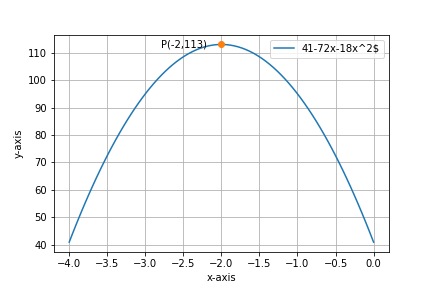
\includegraphics[width=\columnwidth]{solutions/su2021/2/2/assignment14.png}
    \caption{$p(x)=41-72x-18x^2$}
    \label{opt/2/2/p(x)}	
\end{figure}


